\documentclass{beamer}
\usetheme{metropolis} % Use metropolis theme





\title{ECON 3818: Introduction to Statistics with Computer Applications}
%\subtitle
\date{\today}
\author{Kyle Butts}



\definecolor{blue}{RGB}{0,114,178}

\definecolor{red}{HTML}{EB0E09}
\definecolor{yellow}{RGB}{240,228,66}
\definecolor{green}{RGB}{0,158,115}
\definecolor{maroon}{HTML}{AF3335}
\definecolor{purple}{HTML}{7E90B8}


\definecolor{mybackground}{HTML}{ECECEC}
\setbeamercolor{background canvas}{bg= mybackground}

\definecolor{buff-gold}{HTML}{CFB87C}
\definecolor{buff-grey}{HTML}{565A5C}
\definecolor{buff-lightgrey}{HTML}{A2A4A3}
\definecolor{buff-black}{HTML}{000000}

\setbeamercolor{alerted text}{fg=buff-gold!80!black}
\setbeamercolor{frametitle}{bg=buff-black}
\setbeamercolor{title}{fg=buff-grey}
\setbeamercolor{button}{bg=buff-gold}

% Allow to remove indent w/ \begin{itemize}[leftmargin= *]
\usepackage{enumitem}
\setlist[itemize]{label= \textbullet}


% \usepackage[libertine]{newtxmath}
\usepackage{longtable}
\usepackage{booktabs}







\begin{document}



% Title Page ---------------------------------------
\maketitle


% Chapter 2 ----------------------------------------
\section{Chapter 2: Describing Distribution with Numbers}

\begin{frame}{Chapter Overview}
	
	\begin{itemize}
		\item Population vs. Sample
		\item Measures of Central Tendency
		      \begin{itemize}
		      	\item Mean
		      	\item Median
		      \end{itemize}
		\item Measures of Variability
		      \begin{itemize}
		      	\item Quartiles
		      	\item Variance \& Standard Deviation
		      \end{itemize}
	\end{itemize}
	
\end{frame}

\begin{frame}{Population vs Sample}
	
	\begin{itemize}
		\item \alert{Population}: the entire entities under the study
		      \begin{itemize}
		      	\item Examples: all men, all NBA players, all children under 5
		      \end{itemize}
		\item \alert{Sample}: subset of the population
		      \begin{itemize}
		      	\item Can be used to draw inferences about the population
		      	\item Examples: our class, Denver Nuggets players, daycares in Colorado
		      \end{itemize}
		\item Interested in parameters of the population distribution, we can estimate these parameters using data from samples since finding population parameters is infeasible
	\end{itemize}
\end{frame}

\begin{frame}{Population Inference}
	The following graph depicts the underlying population distribution
	\begin{itemize}
		\item We are interested in its parameters, but are unable collect data on every simple observation
	\end{itemize}
	\begin{center}
		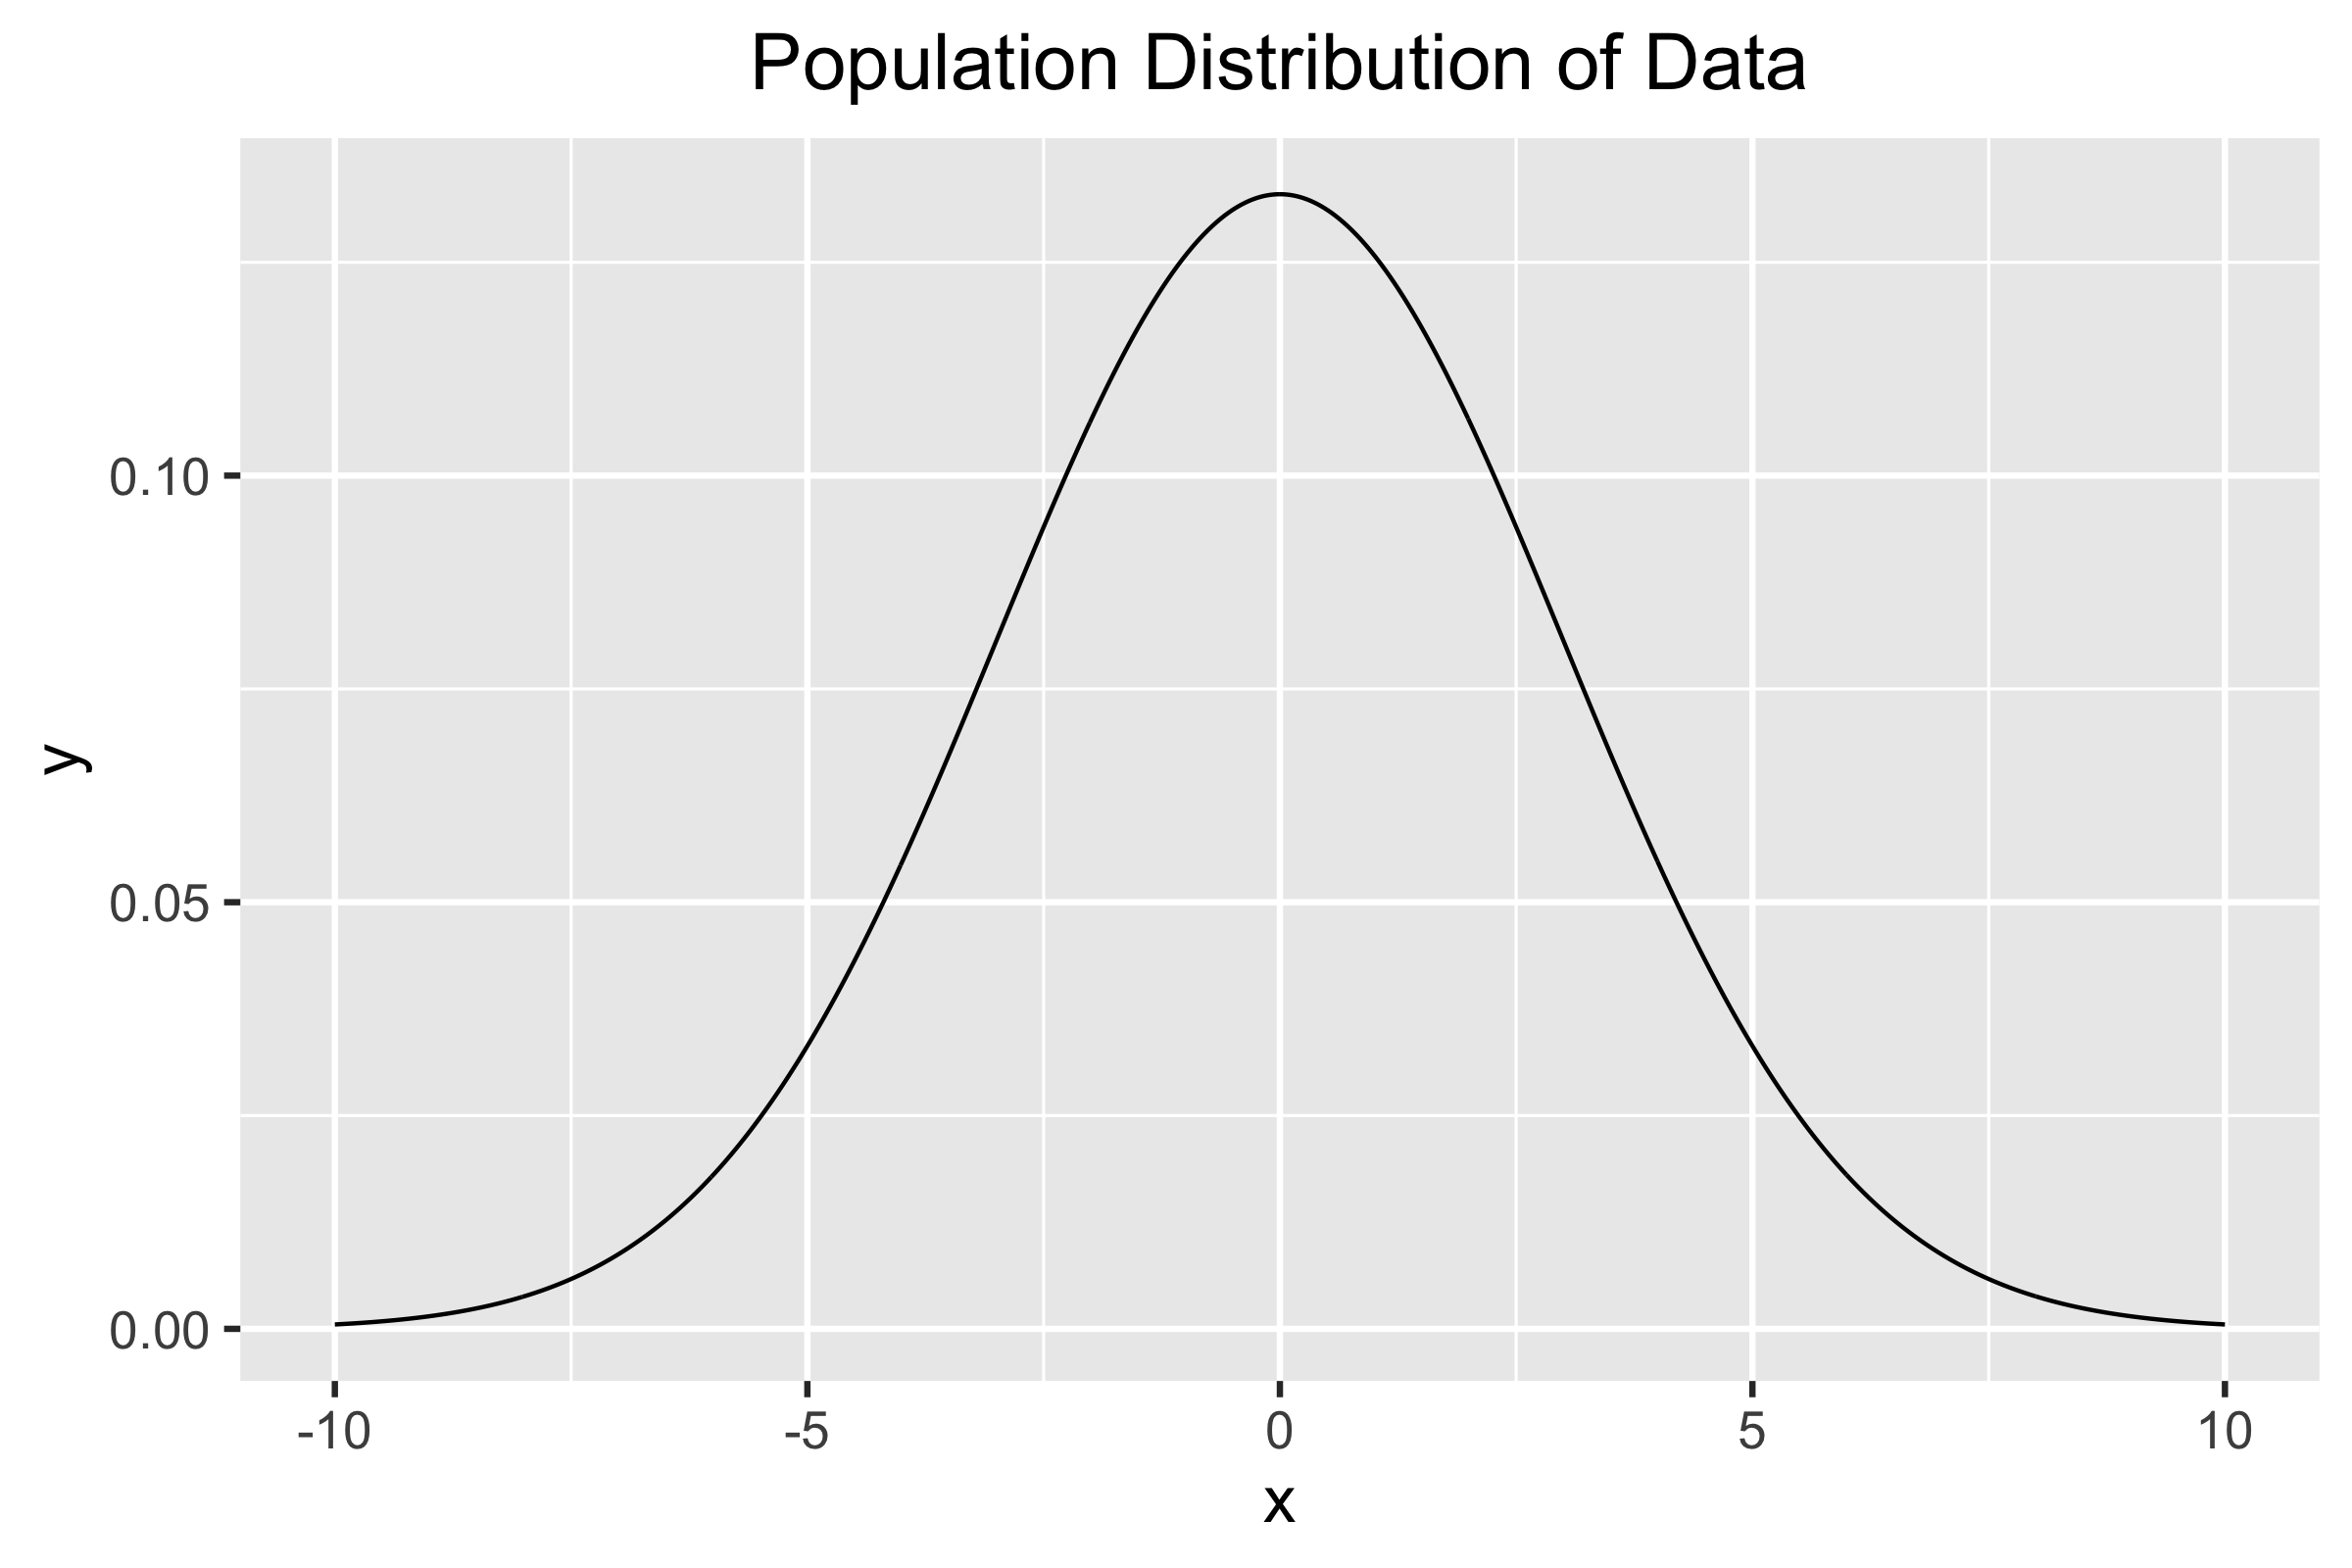
\includegraphics[width=0.65\textwidth]{normdistn}
	\end{center}
\end{frame}

\begin{frame}{Population Inference}
	What we do instead is use a sample of the population and use that sample distribution to determine parameters of interest
	\begin{center}
		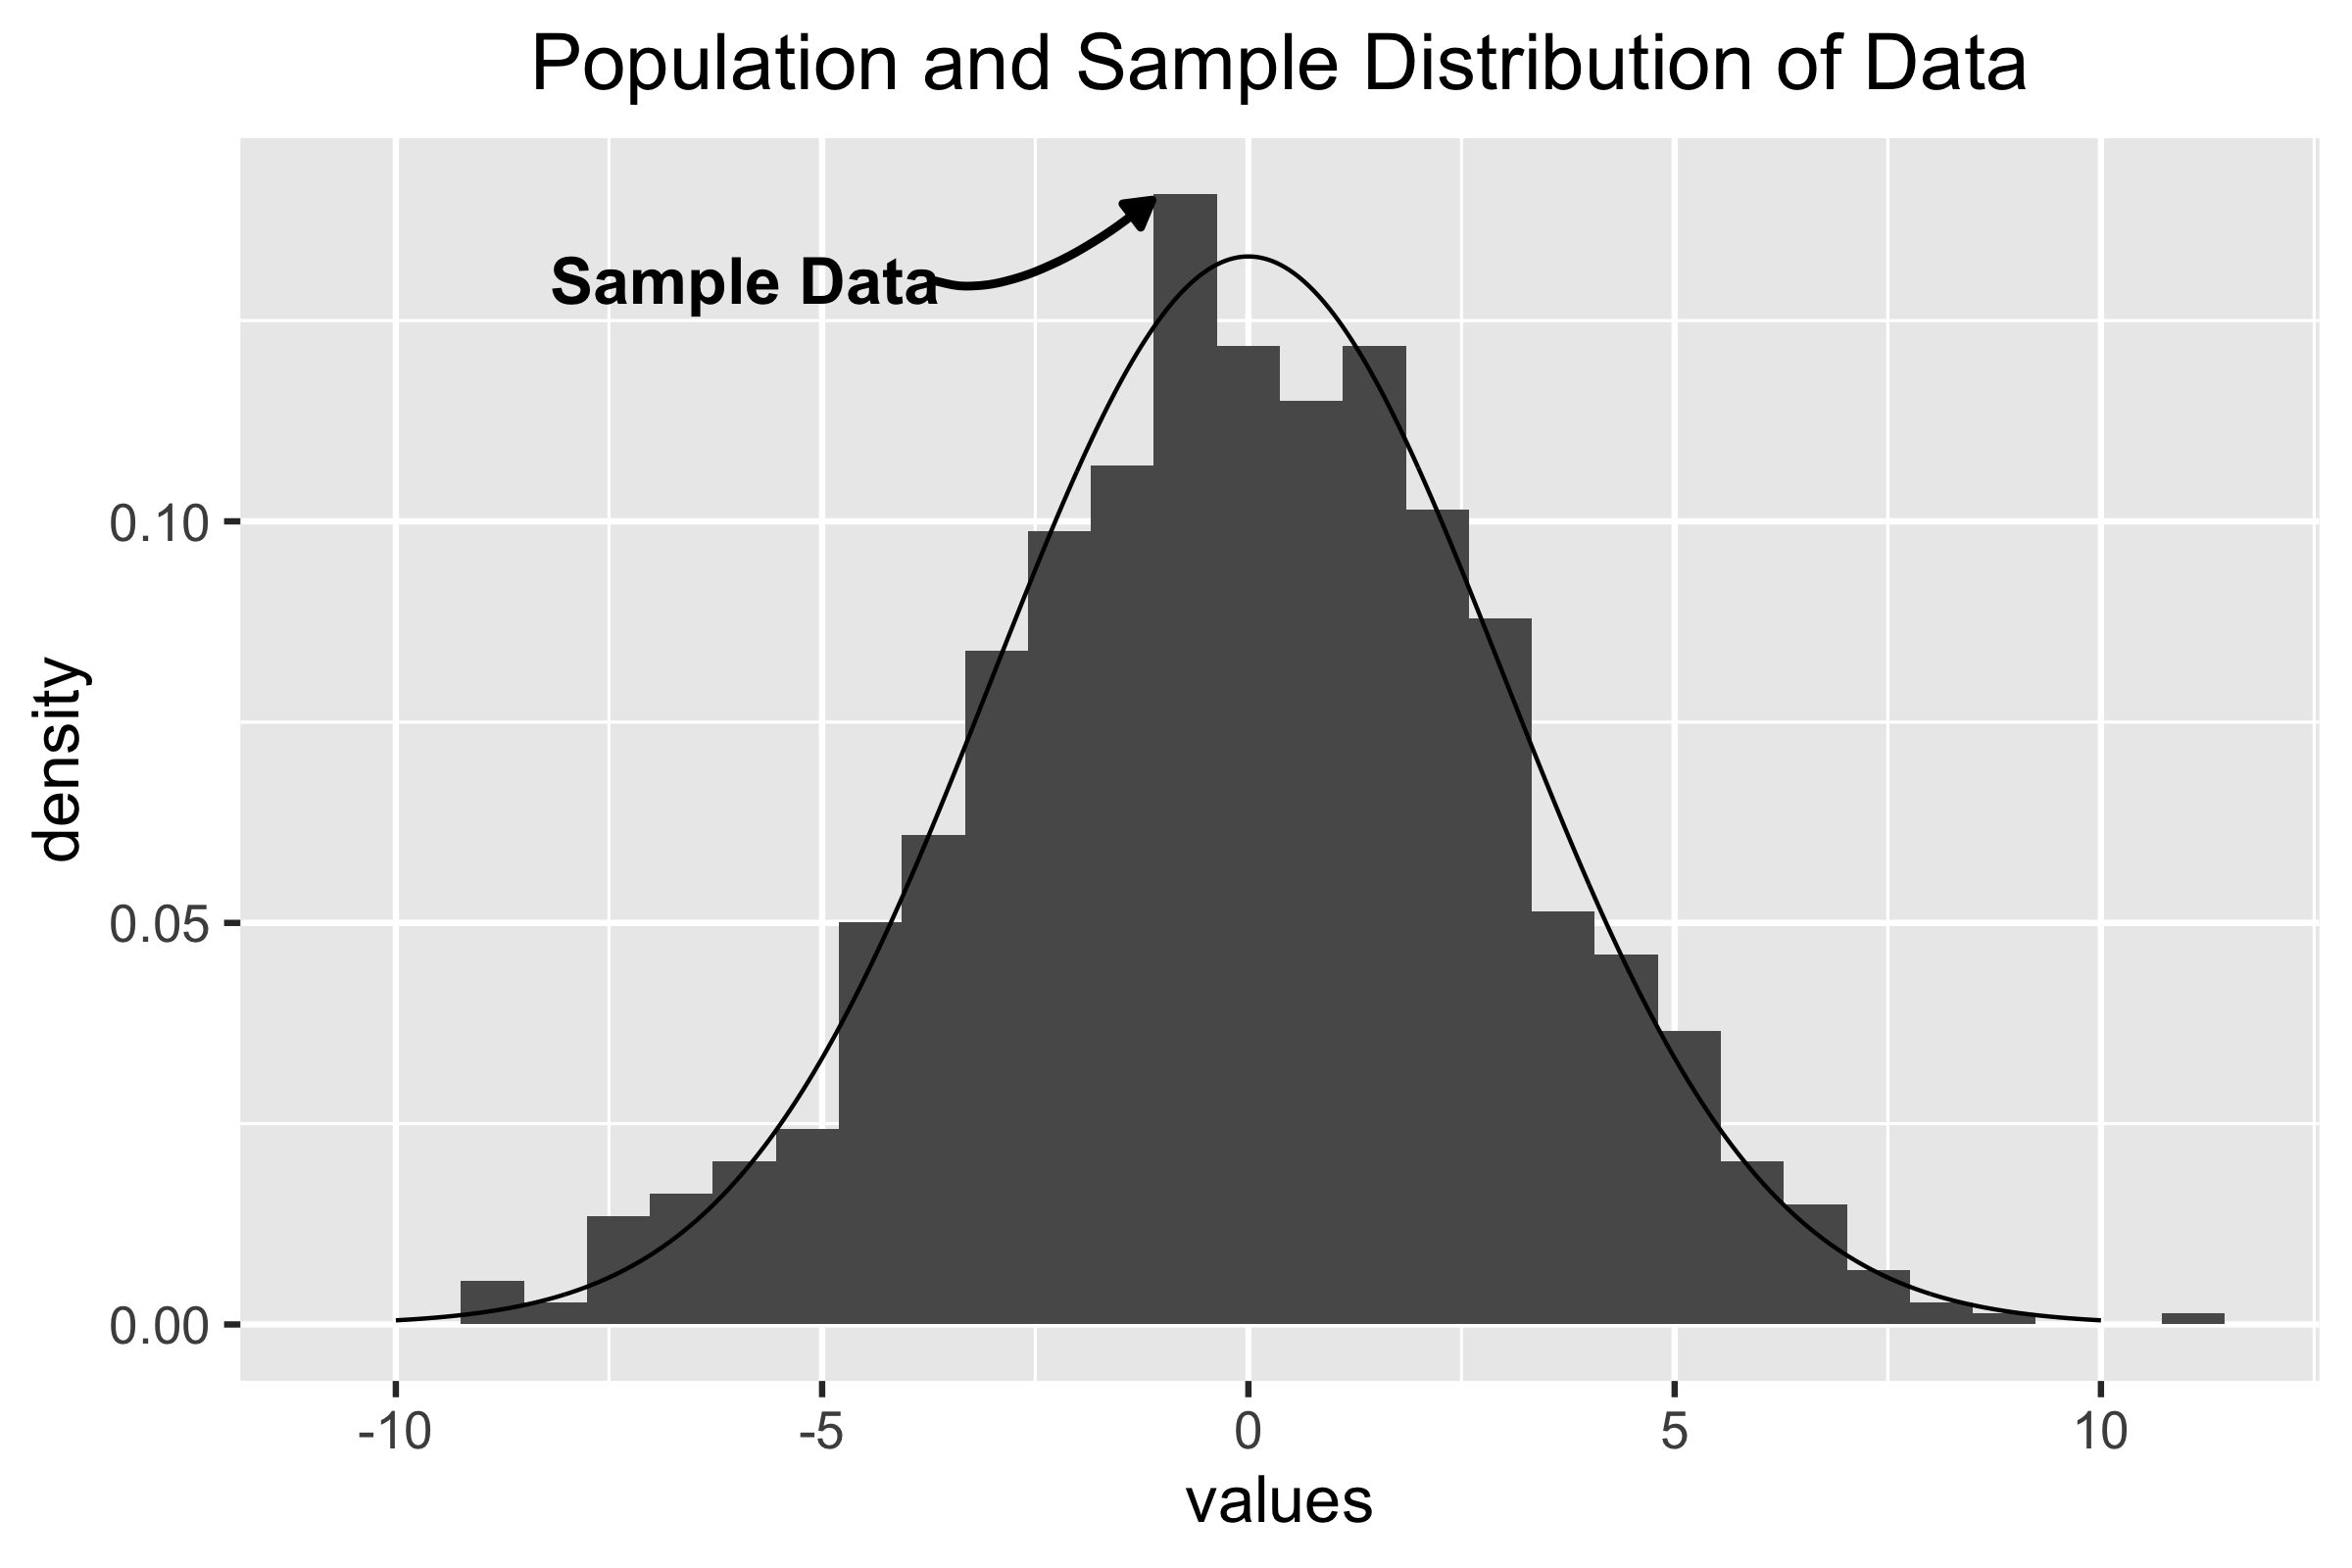
\includegraphics[width=0.7\textwidth]{normdistnsamplehist}
	\end{center}
\end{frame}


\begin{frame}{Parameters of Interest}
	
	\begin{itemize}
		\item Two primary population parameters of interest:
		      \begin{itemize}
		      	\item Measures of central tendency
		      	      \begin{itemize}
		      	      	\item Population mean, $\mu$
		      	      \end{itemize}
		      	\item Measures of variability 
		      	      \begin{itemize}
		      	      	\item Population variance, $\sigma^2$
		      	      \end{itemize}
		      \end{itemize}
		\item We will estimate these using the sample distribution
	\end{itemize}
	
\end{frame}

\begin{frame}{Measuring Center}
	
	\begin{itemize}
		\item Measures of central tendency tells us about some center value of a distribution
		      \begin{itemize}
		      	\item Mean
		      	\item Median
		      \end{itemize}
	\end{itemize}
	
\end{frame}

\begin{frame}{Measuring Center: the Mean}
	
	\begin{itemize}
		\item The most common measure of center is the arithmetic average, or \alert{mean}
		      $$\bar{x}= \frac{x_1 + x_2 + .... + x_n}{n}$$
		      or more compactly:
		      $$\bar{x}=\frac{1}{n}\sum x_i$$
	\end{itemize}
	
\end{frame}

\begin{frame}{Measuring Center: the Median}
	
	\begin{itemize}
		\item The \alert{median} is the midpoint of a distribution
		      \begin{itemize}
		      	\item Is more resistant to the influence of extreme observations 
		      \end{itemize}
		\item How to calculate median:
		      \begin{itemize}
		      	\item Arrange observations from smallest to largest
		      	\item If there is odd number of observations, the median is the center observation. If there are even number of observations, the median is the average of two center observations
		      \end{itemize}
	\end{itemize}
\end{frame}

\begin{frame}{Mean vs. Median}
	
	\begin{itemize}
		\item Although we will primarily be using the mean throughout the semester, the biggest drawback of the mean is that it is not resistant to outliers
		      
		\item The median, however, is resistant to outliers so it can be important to calculate for smaller samples 
	\end{itemize}
	
\end{frame}

%% Do class example
%% Lets say we're looking at salaries for 5 NBA players
%% Include LeBron as an outlier
%% calculate average 
%% calculate median
%% emphasize that one huge outlier does not affect the median 

\begin{frame}{Clicker Question}
	\begin{center}
		What is the average age of the participants?
		\vskip.25in
		\begin{tabular}{ | c | c | c | c |}
			\hline
			\textbf{Age} & \textbf{Sex} & \textbf{BMI} & \textbf{Drinks per week} \\ [0.5ex]
			\hline
			59           & male         & 32.26        & 3 drinks                 \\
			\hline
			62           & male         & 25.09        & 2 drinks                 \\
			\hline
			60           & female       & 32.58        & 1 drink                  \\ 
			\hline
			18           & male         & 99.99        & 6 drinks                 \\ 
			\hline
			57           & female       & 31.88        & 2 drinks                 \\ 
			\hline
			56           & male         & 42.8         & 3 drinks                 \\
			\hline
		\end{tabular}

		\begin{enumerate}[label=(\alph*)]
			\item 58
			\item 51.2
			\item 52
			\item 49.7
		\end{enumerate}
	\end{center}
\end{frame}

\begin{frame}{Clicker Question}
	\begin{center}
		Which measure of central tendency best describes the age of participants?
		
		\begin{tabular}{ | c | c | c | c |}
			\hline
			\textbf{Age} & \textbf{Sex} & \textbf{BMI} & \textbf{Drinks per week} \\ [0.5ex]
			\hline
			59           & male         & 32.26        & 3 drinks                 \\
			\hline
			62           & male         & 25.09        & 2 drinks                 \\
			\hline
			60           & female       & 32.58        & 1 drink                  \\ 
			\hline
			18           & male         & 99.99        & 6 drinks                 \\ 
			\hline
			57           & female       & 31.88        & 2 drinks                 \\ 
			\hline
			56           & male         & 42.8         & 3 drinks                 \\
			\hline
		\end{tabular}
		\begin{enumerate}[label=(\alph*)]
			\item Mean
			\item Median
		\end{enumerate}
	\end{center}
\end{frame}




\begin{frame}{Measuring Variability}
	
	\begin{itemize}
		\item Measures of central tendency do not tell the whole story. To further characterize the distribution, we need to know how the data is spread out
		      \begin{itemize}
		      	\item Quartiles
		      	\item Variance
		      \end{itemize}
	\end{itemize}
	
\end{frame}


\begin{frame}{Measuring Variability: Quartiles}
	
	\begin{itemize}
		\item Measure of center alone can be misleading
		\item How to calculate quartiles:
		      \begin{itemize}
		      	\item Arrange observations in increasing order and locate median 
		      	\item The \alert{first quartile} is the median of the observations located to the left of the median
		      	\item The \alert{third quartile} is the median of observations located to the right of the median
              \end{itemize}
              
		      \begin{center}
		      	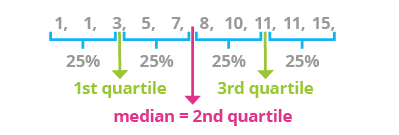
\includegraphics[width=0.8\textwidth]{quartiles}
		      \end{center}
		      
	\end{itemize}
\end{frame}


%% Do another board example of calculating quartiles

\begin{frame}{Boxplots}
	\begin{itemize}
		\item \alert{five-number summary}: smallest observation (minimum), the first quartile, the median, the third quartile, and the largest observation (maximum)
		\item We can use the \alert{boxplot} using this five number summary to display quantitative data
		\item How to make a boxplot:
		      \begin{itemize}
		      	\item A central box spans the first and third quartiles 
		      	\item A line in the box marks the median
		      	\item Line extends from the box out to the smallest and largest observations 
		      \end{itemize}
	\end{itemize}
\end{frame}

\begin{frame}{Boxplots}
	
	\begin{center}
		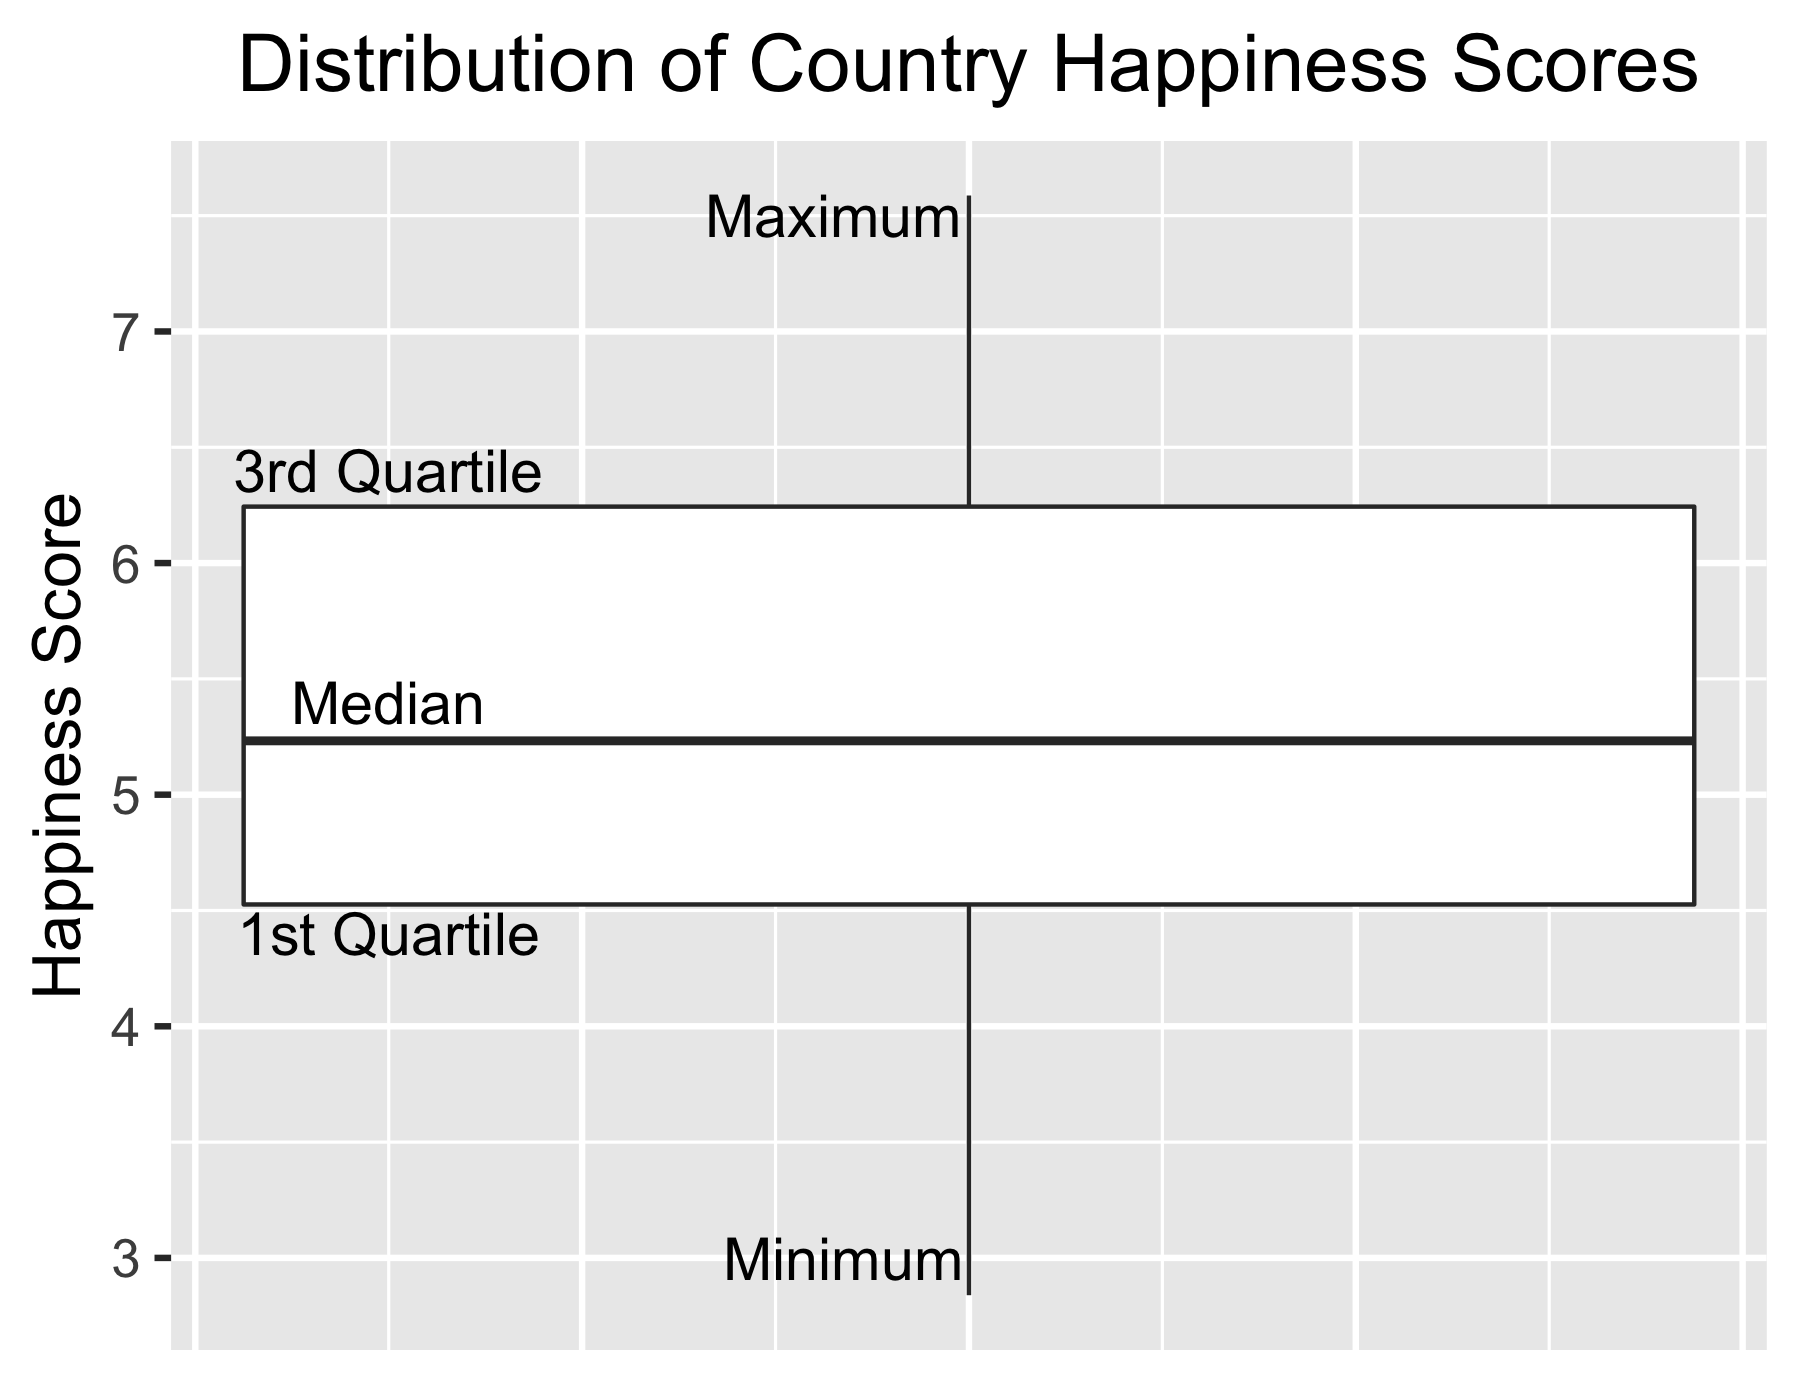
\includegraphics[width=0.8\textwidth]{boxplot}
	\end{center}
	\small{Data provided by the UN's World Happiness Report}
\end{frame}

\begin{frame}{Boxplots}
	
	\begin{center}
		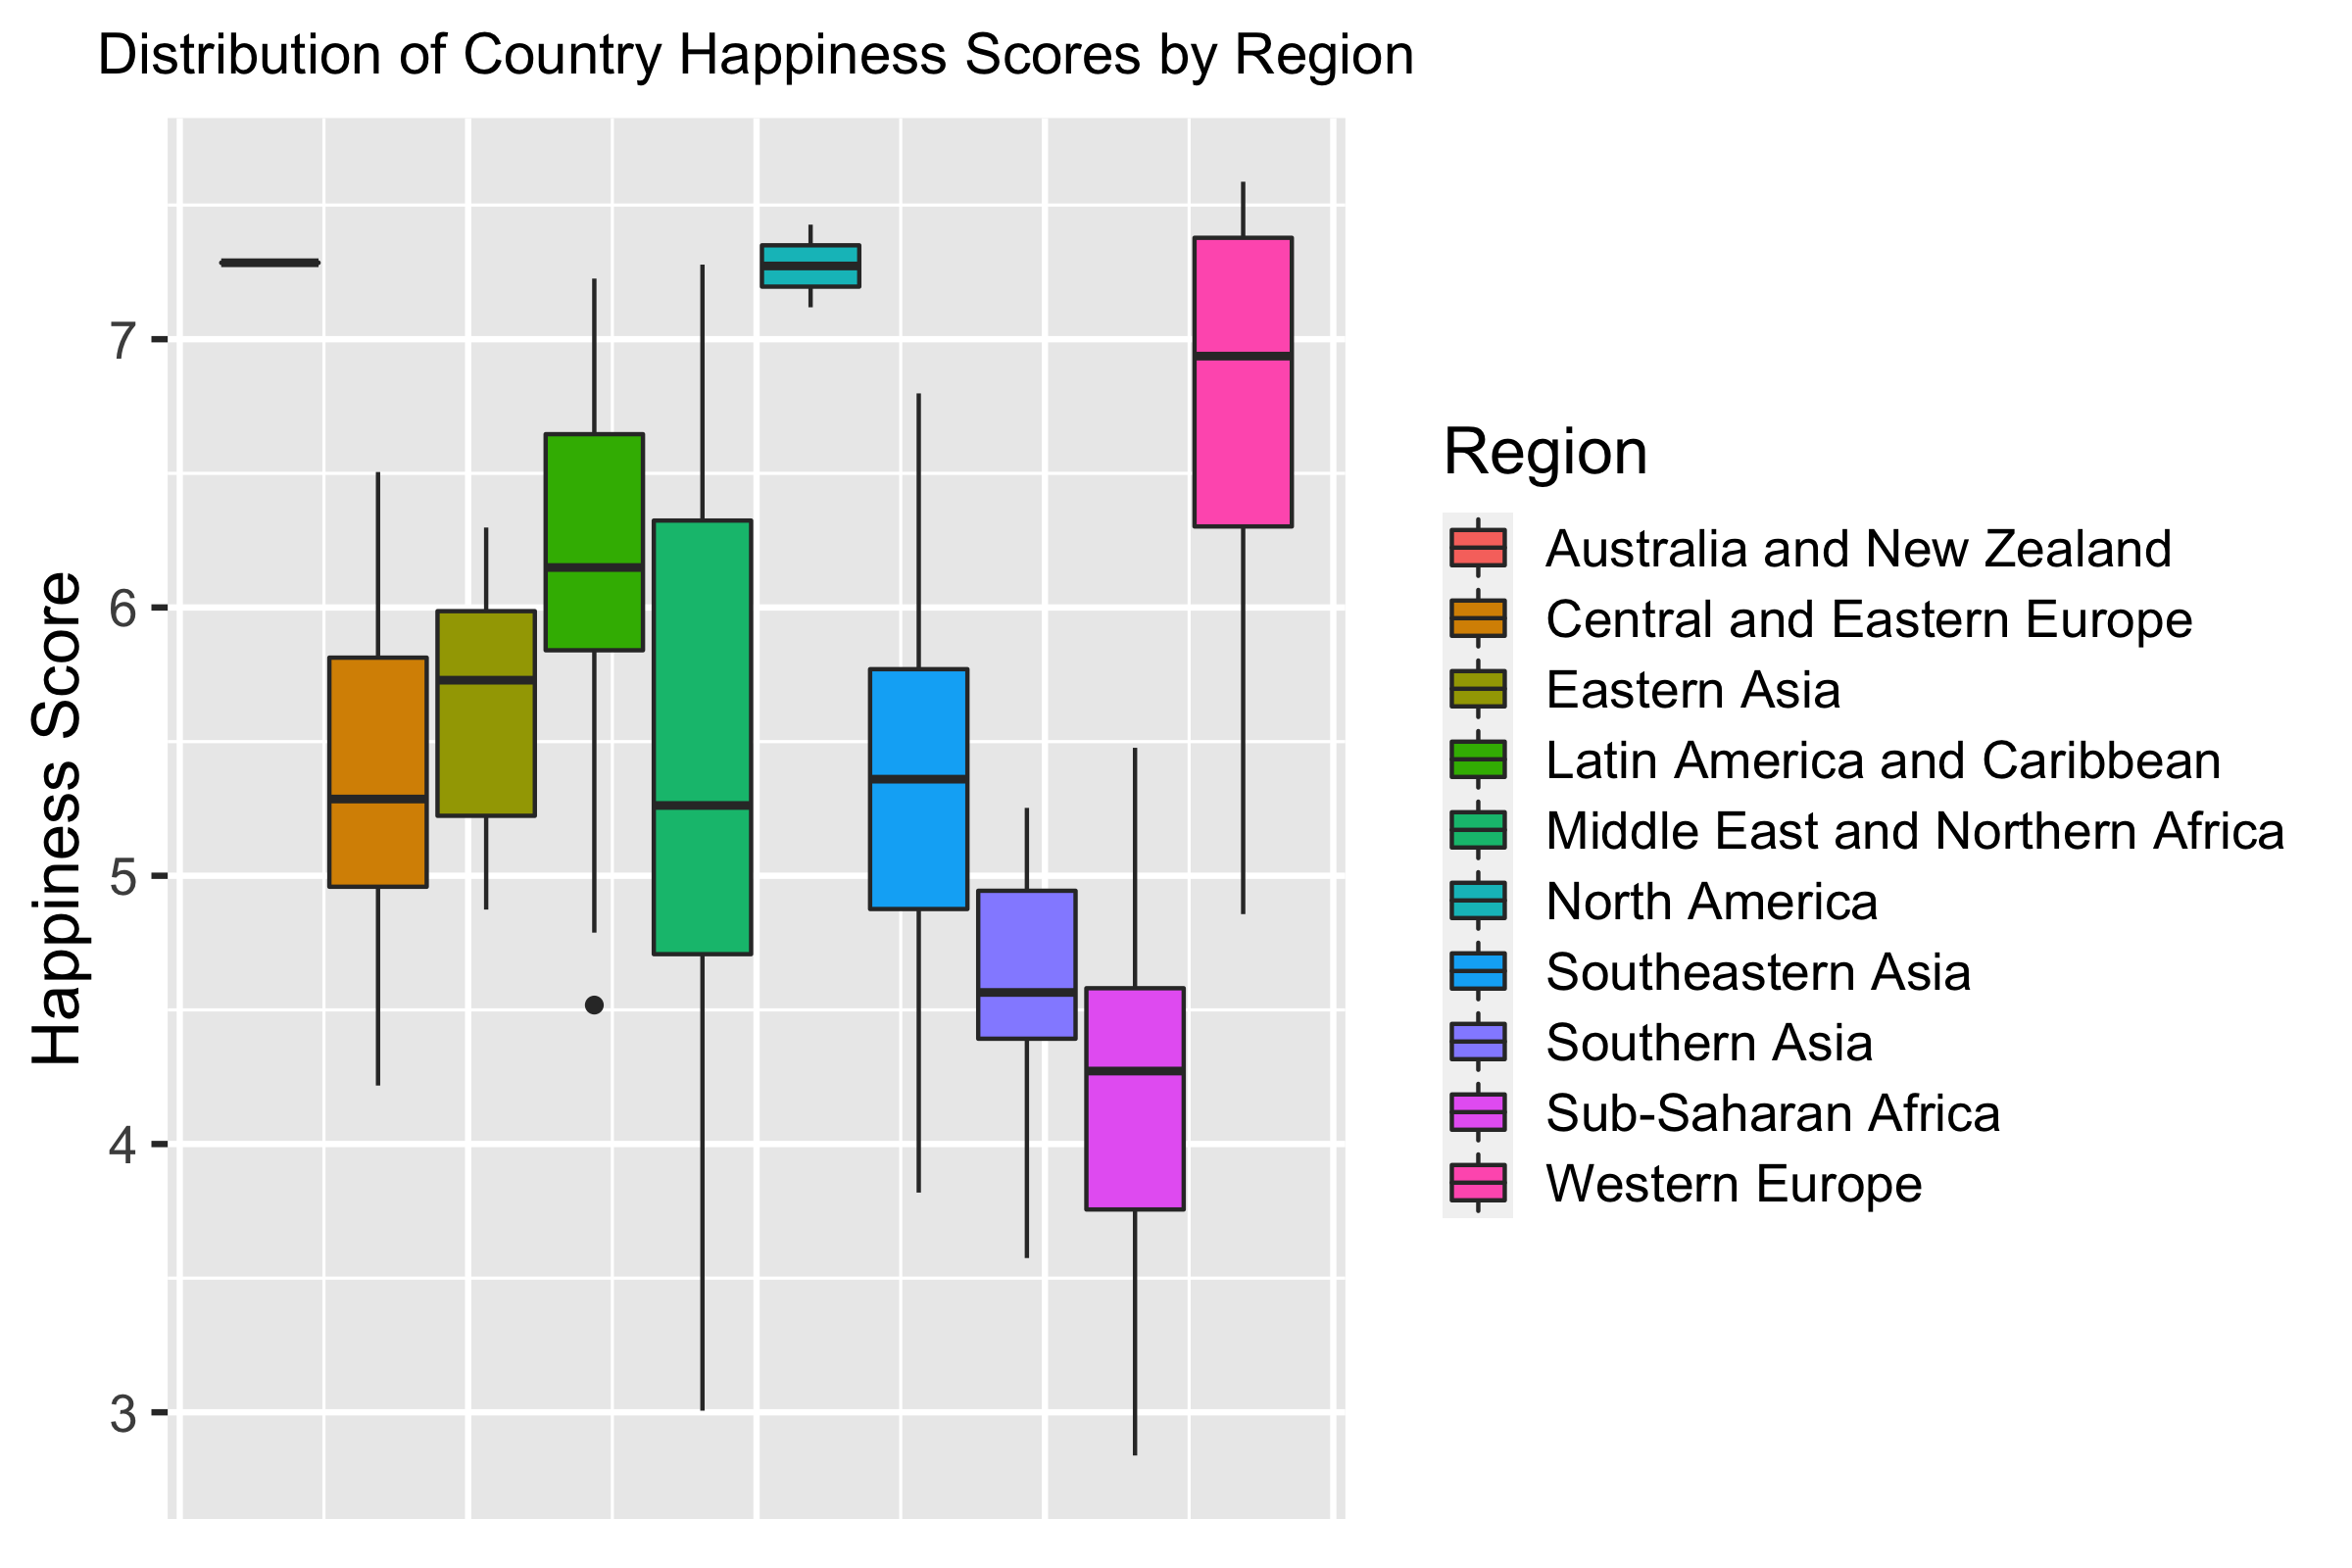
\includegraphics[width=\textwidth]{boxplot_region}
	\end{center}
	\small{Data provided by the UN's World Happiness Report}
\end{frame}

%% bocplot example 
%% purple box is men -- see that the purple box is "higher" than green box on all days except Sat
%% meaning, men spend more on bills Thursday, Friday, and a bit on Sunday
%% whiskers are long on the male boxplots -- how much men spend on the data varies more than how mich women spend 

\begin{frame}{Interquartile Range}
	
	\begin{itemize}
		\item The \alert{interquartile range}, IQR, is the distance between the first and third quartiles
		      \begin{itemize}
		      	\item IQR = $Q_3 - Q_1$
		      	\item The IQR measures the spread
		      	\item It also helps to identify outliers
		      \end{itemize}
		\item Rule for outliers:
		      \begin{itemize}
		      	\item An observation is an outlier if it falls more than 1.5 x IQR above the third quartile or below the first
		      \end{itemize}
	\end{itemize}
	
\end{frame}




\begin{frame}{Measuring Variability: Variance}
	
	\begin{itemize}
		\item \alert{Variance}: denoted, $s^2$, measures how "spread out" the data are on average
		      $$s^2 = \frac{(x_1-\bar{x})^2 + (x_2-\bar{x})^2 + .... + (x_n - \bar{x})^2}{n-1}$$
	\end{itemize}
	
\end{frame}

\begin{frame}{Measuring Variability: Standard Deviation}
	
	\begin{itemize}
		\item \alert{Standard deviation}: looks at how far each observation is from the mean; square root of the variance
		      $$s=\sqrt{\frac{1}{n-1}\sum_{i=1}^n(x_i-\bar{x})^2}$$
	\end{itemize}
	
\end{frame}

\begin{frame}{Visualizing Standard Deviation}
	\begin{center}
		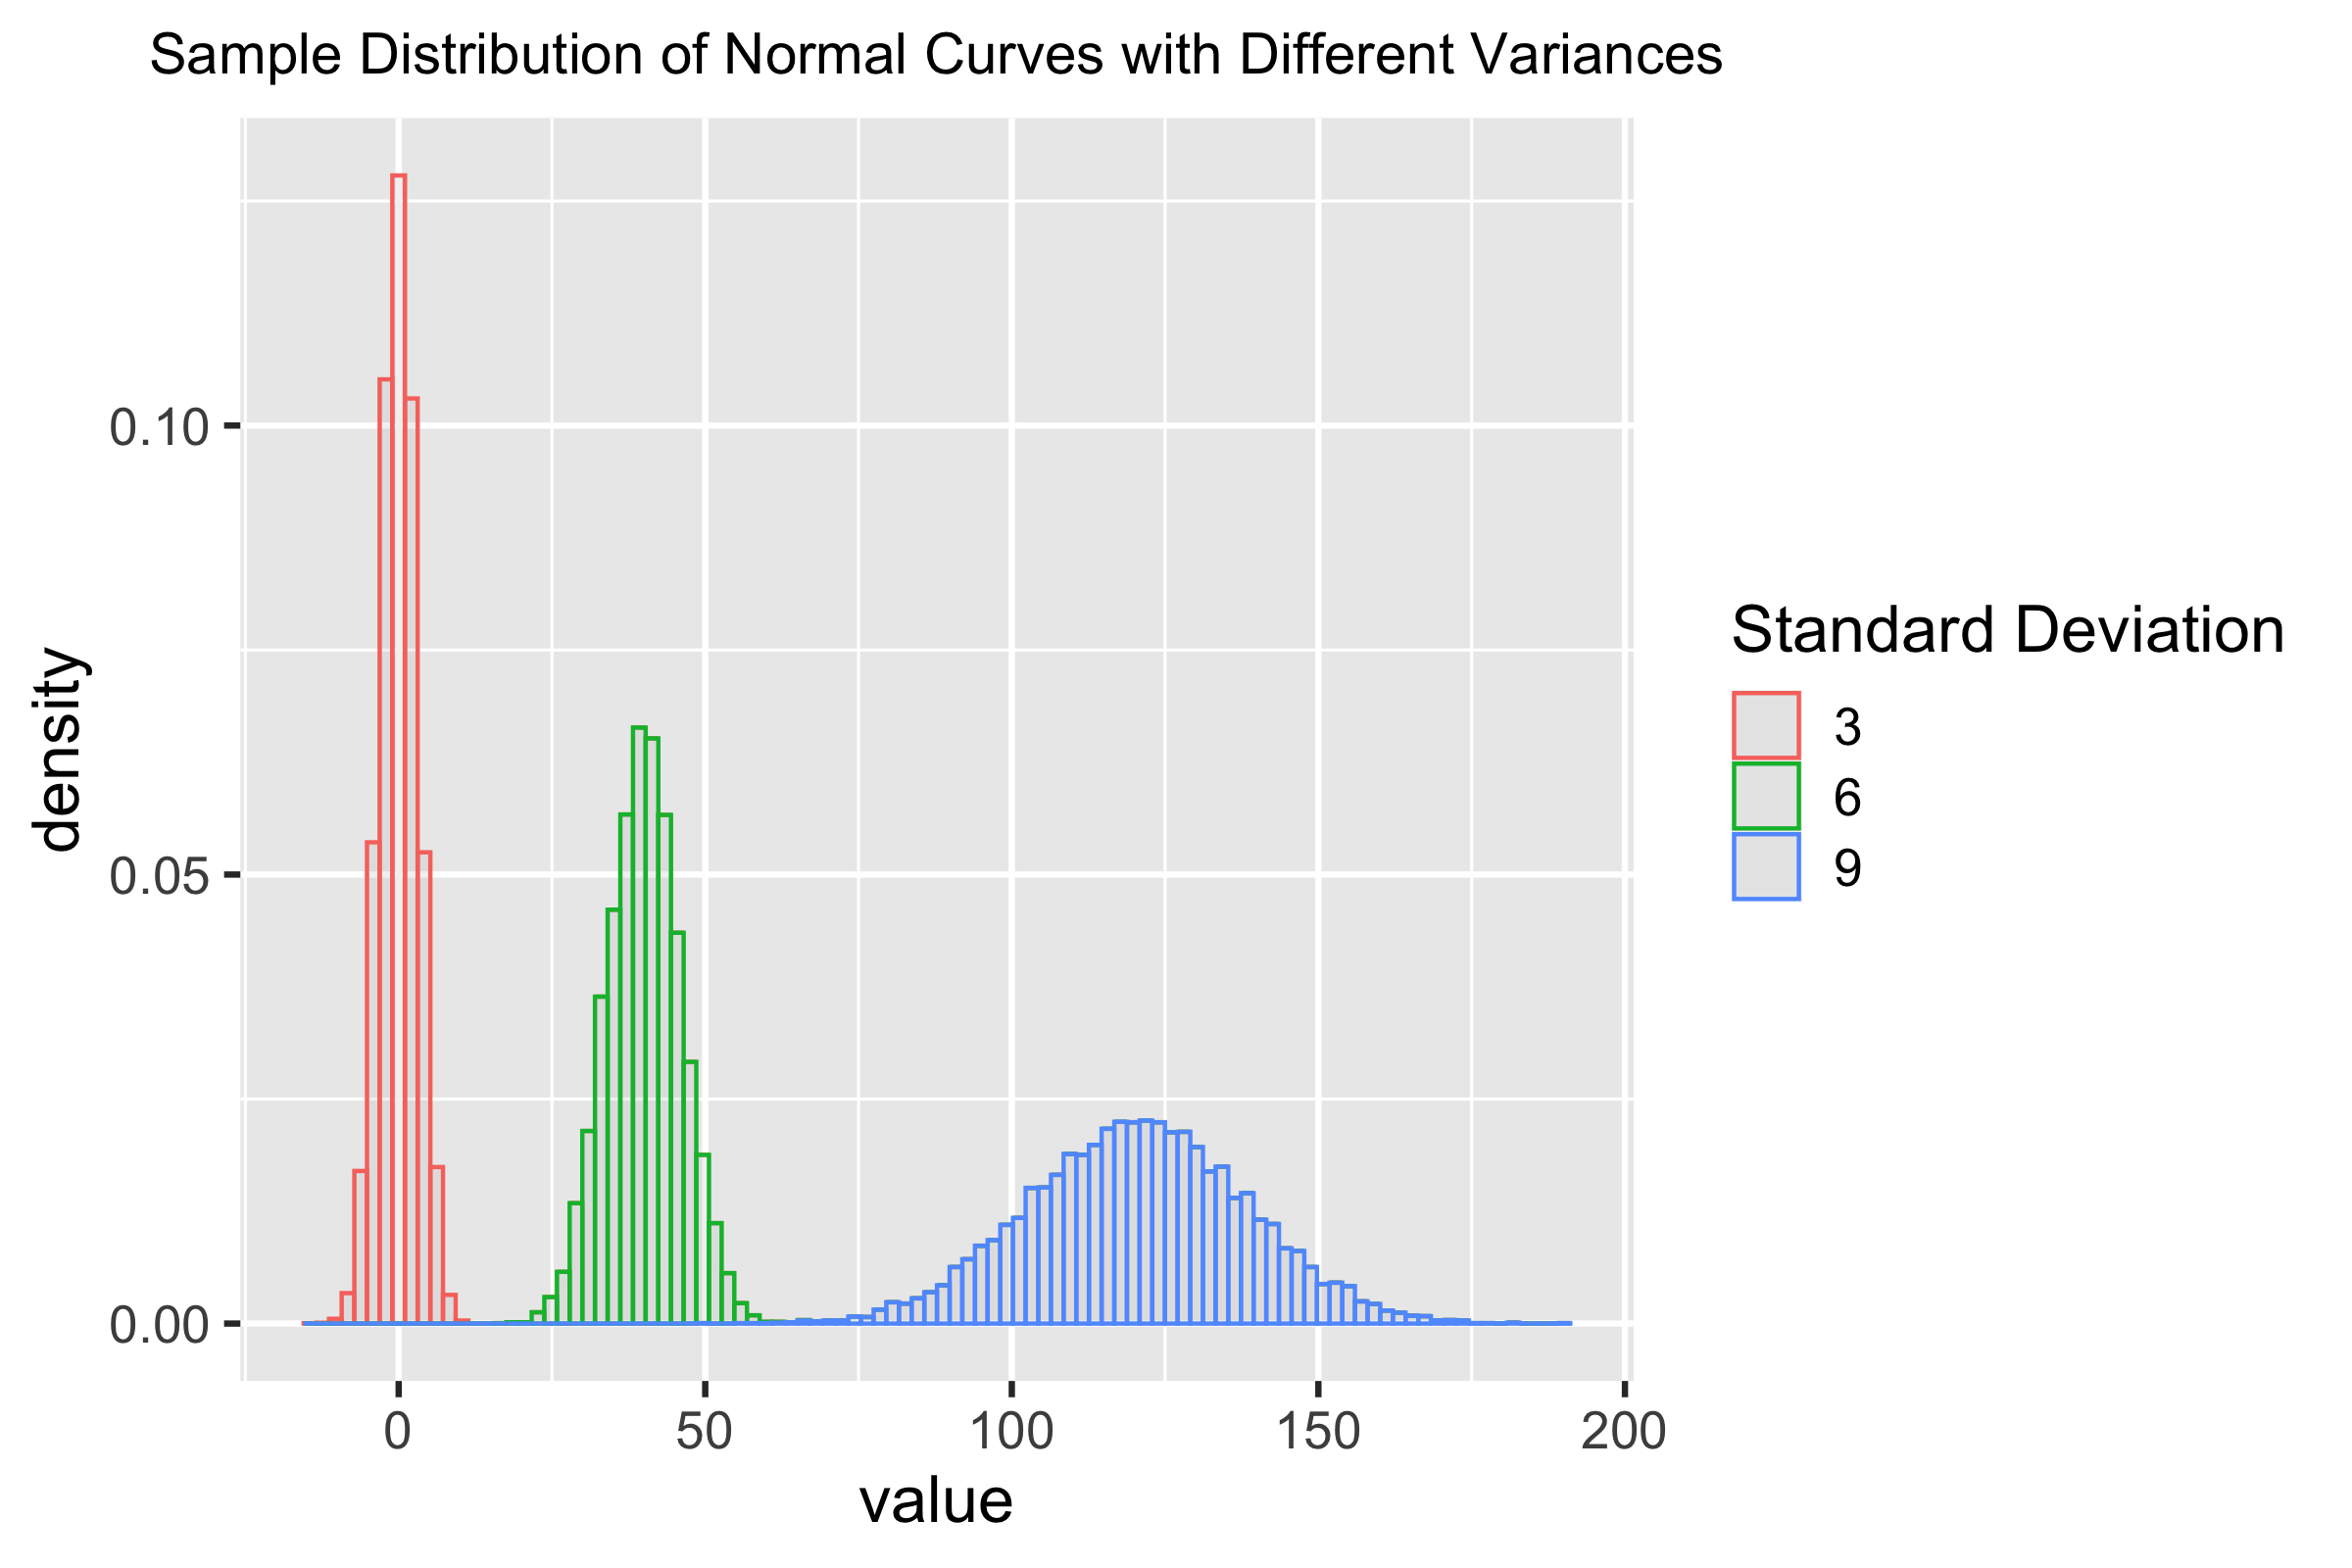
\includegraphics[width=\linewidth]{normdist_multiplevars.png}
	\end{center}
\end{frame}


%% turn this into clicker question?
\begin{frame}{Practice Question}
	
	Calculate the standard deviation of age?
	\begin{center}
		\begin{tabular}{ | c | c | c | c |}
			\hline
			\textbf{Age} & \textbf{Sex} & \textbf{BMI} & \textbf{Drinks per week} \\ [0.5ex]
			\hline
			59           & male         & 32.26        & 3 drinks                 \\
			\hline
			62           & male         & 25.09        & 2 drinks                 \\
			\hline
			60           & female       & 32.58        & 1 drink                  \\ 
			\hline
			18           & male         & 99.99        & 6 drinks                 \\ 
			\hline
			57           & female       & 31.88        & 2 drinks                 \\ 
			\hline
		\end{tabular}
	\end{center}
\end{frame}





\begin{frame}{Properties of $s$}
	
	\begin{itemize}
		\item $n-1$ is referred to as the degrees of freedom
		\item $s$ measures variability about the mean
		\item $s$ is always greater than or equal to zero, but usually $> 0$
		\item As observations become more variable, $s$ gets larger
		\item $s$ is not resistant in the same way the sample mean is not resistant; a few outliers can change it a lot.
	\end{itemize}
	
\end{frame}

\begin{frame}{Summary of Summary Statistics}
	Two basic ways to summarize the center and spread of a distribution
	\begin{itemize}
		\item Mean and standard deviation (or variance)
		\item The five-number summary
	\end{itemize}

	When $\bar{x}$ and $s$ are good measures (i.e. they aren't too affected by outliers)
	\begin{itemize}
		\item Use $\bar{x}$ and $s$ when the distribution is reasonably symmetric and free of outliers
		      \begin{itemize}
		      	\item Most commonly used approach
		      \end{itemize}
		\item Use five-number summary if distribution is skewed, or has outliers
	\end{itemize}
\end{frame}



\begin{frame}{Greek Letters and Statistics}
	\begin{columns}[onlytextwidth] % align columns

		\begin{column}{.5\textwidth}
			\begin{center}
				\textbf{Greek Letters}
			\end{center}

			\begin{itemize}
				\item Greek letters like $\mu$ and $\sigma^2$ represent the truth about the population.
			\end{itemize}
		\end{column}%
		\hfill%

		\begin{column}{.5\textwidth}
			\begin{center}
				\textbf{Latin Letters}
			\end{center}

			\begin{itemize}
				\item Latin lettes like $\bar{x}$ and $s^2$ are calculations that represent guesses (estimates) at the population values.
			\end{itemize}
		\end{column}%
	\end{columns}
	
	\vspace{10mm}
	The goal for the class is for the latin letters to be good guesses for the greek letters:

	\[ 
		\text{Data} \longrightarrow \text{Calculation} \longrightarrow \text{Estimates} \longrightarrow^{hopefully!} \text{Truth}
	\]
	\[
		X \longrightarrow 1/n \sum_{i=1}^n X_i \longrightarrow \bar{x} \longrightarrow^{hopefullly!} \mu
	\]
\end{frame}



\begin{frame}{R Studio}
	
	How to install R \& R Studio
	\begin{itemize}
		\item \url{https://www.r-project.org/}
		\item Click "download R" link under "Getting Started"
		\item Select a CRAN location (mirror site) and click link
		      \begin{itemize}
		      	\item I selected the UC Berkeley one, pick one in USA
		      \end{itemize}
		\item Click on "Download R for Mac/Windows/etc" link at top of page
		\item Click on package to download, under "Latest Release"
		\item Save the .pkg file, double click open, and follow instructions 
		\item \url{www.rstudio.com} and click "Download RStudio"
		\item Click on "download RStudio Desktop"
	\end{itemize}
	
\end{frame}


\begin{frame}{How to use R}
	\begin{center}
		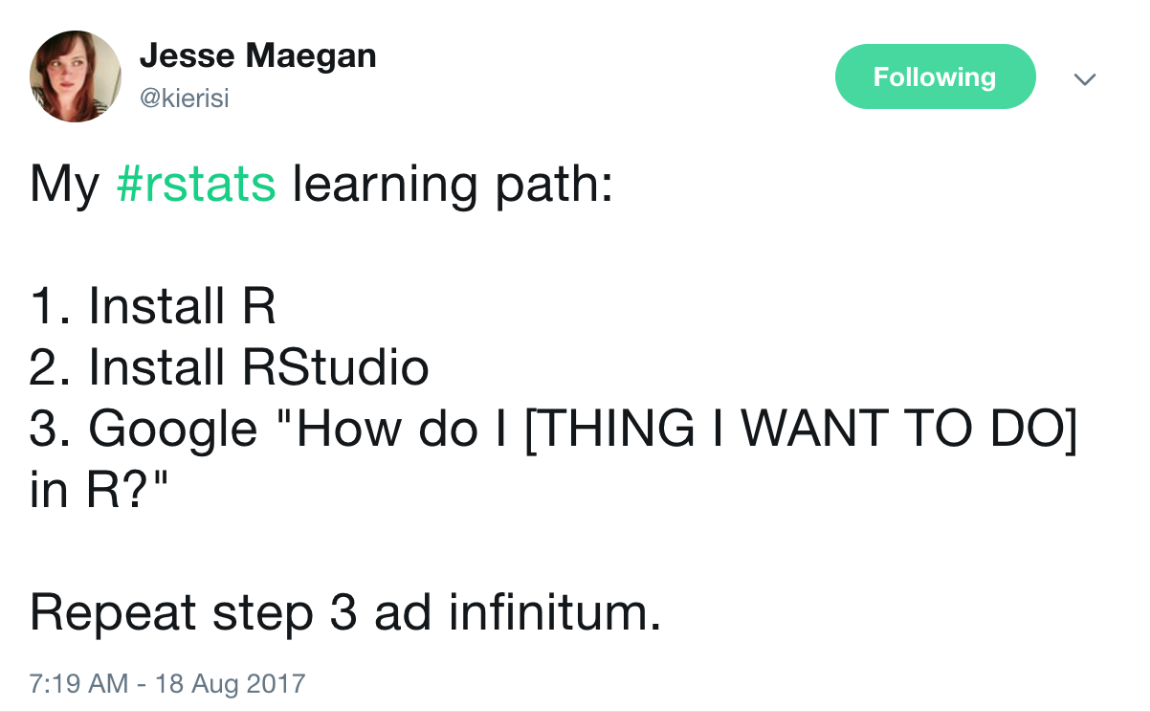
\includegraphics[width=\linewidth]{r.png}
	\end{center}
\end{frame}


% % Extra slides about quartlies (depending how far you want to discuss)
%\begin{frame}{Quartiles -- Odd}
%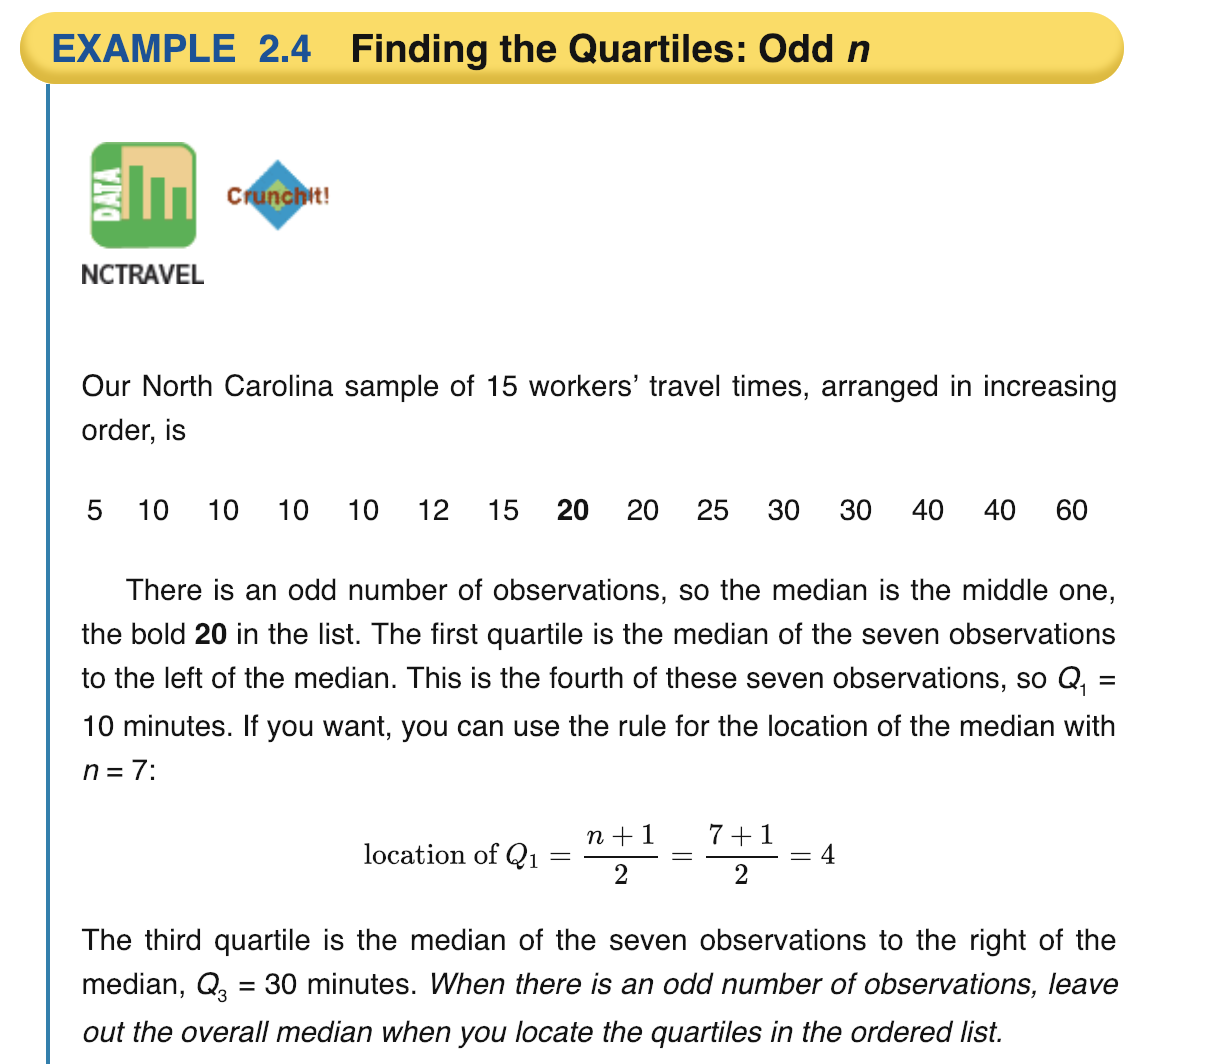
\includegraphics[width=0.78\textwidth]{quartile_odd}
%\end{frame}

%\begin{frame}{Quartiles -- Even}
%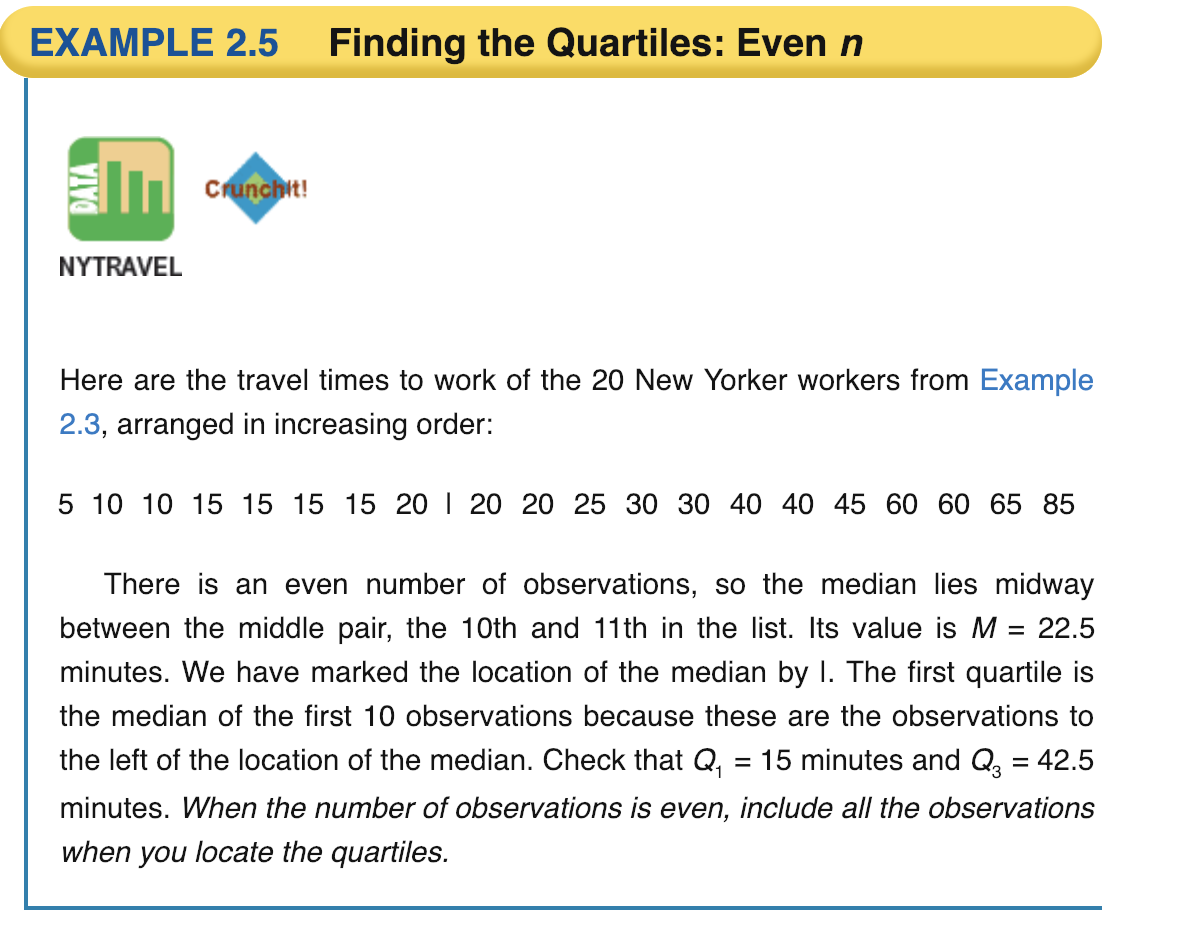
\includegraphics[width=0.8\textwidth]{quartile_even}
%\end{frame}


% % Extra Slides if interested:
%\begin{frame}{Mean/Median}
%\begin{center}
%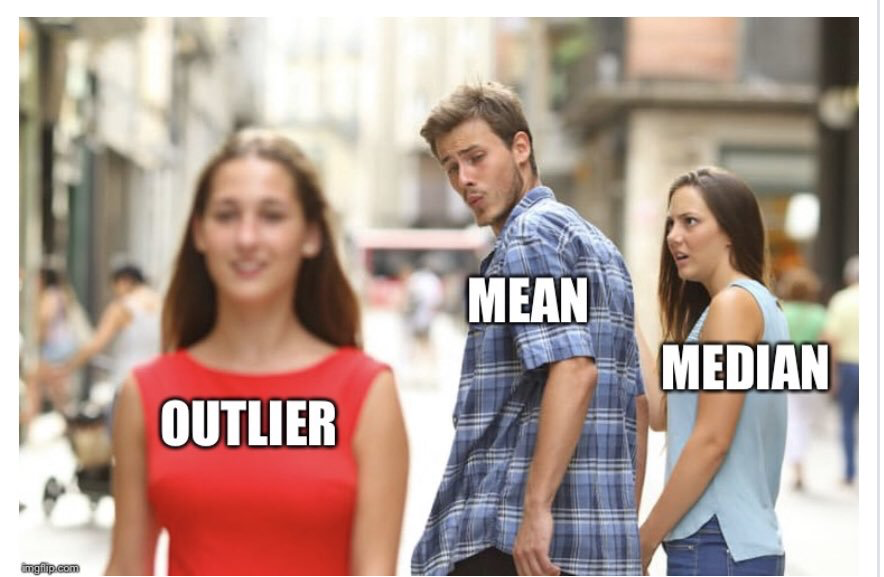
\includegraphics[width=0.75\textwidth]{meme.png}
%\end{center}
%\end{frame}

%\begin{frame}{5 Number Summary \& Histogram}
%\begin{columns}
%\column{0.5\textwidth}
%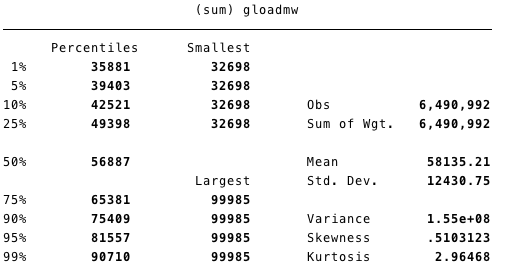
\includegraphics[width=\textwidth]{research_5number}
%\column{0.5\textwidth}
%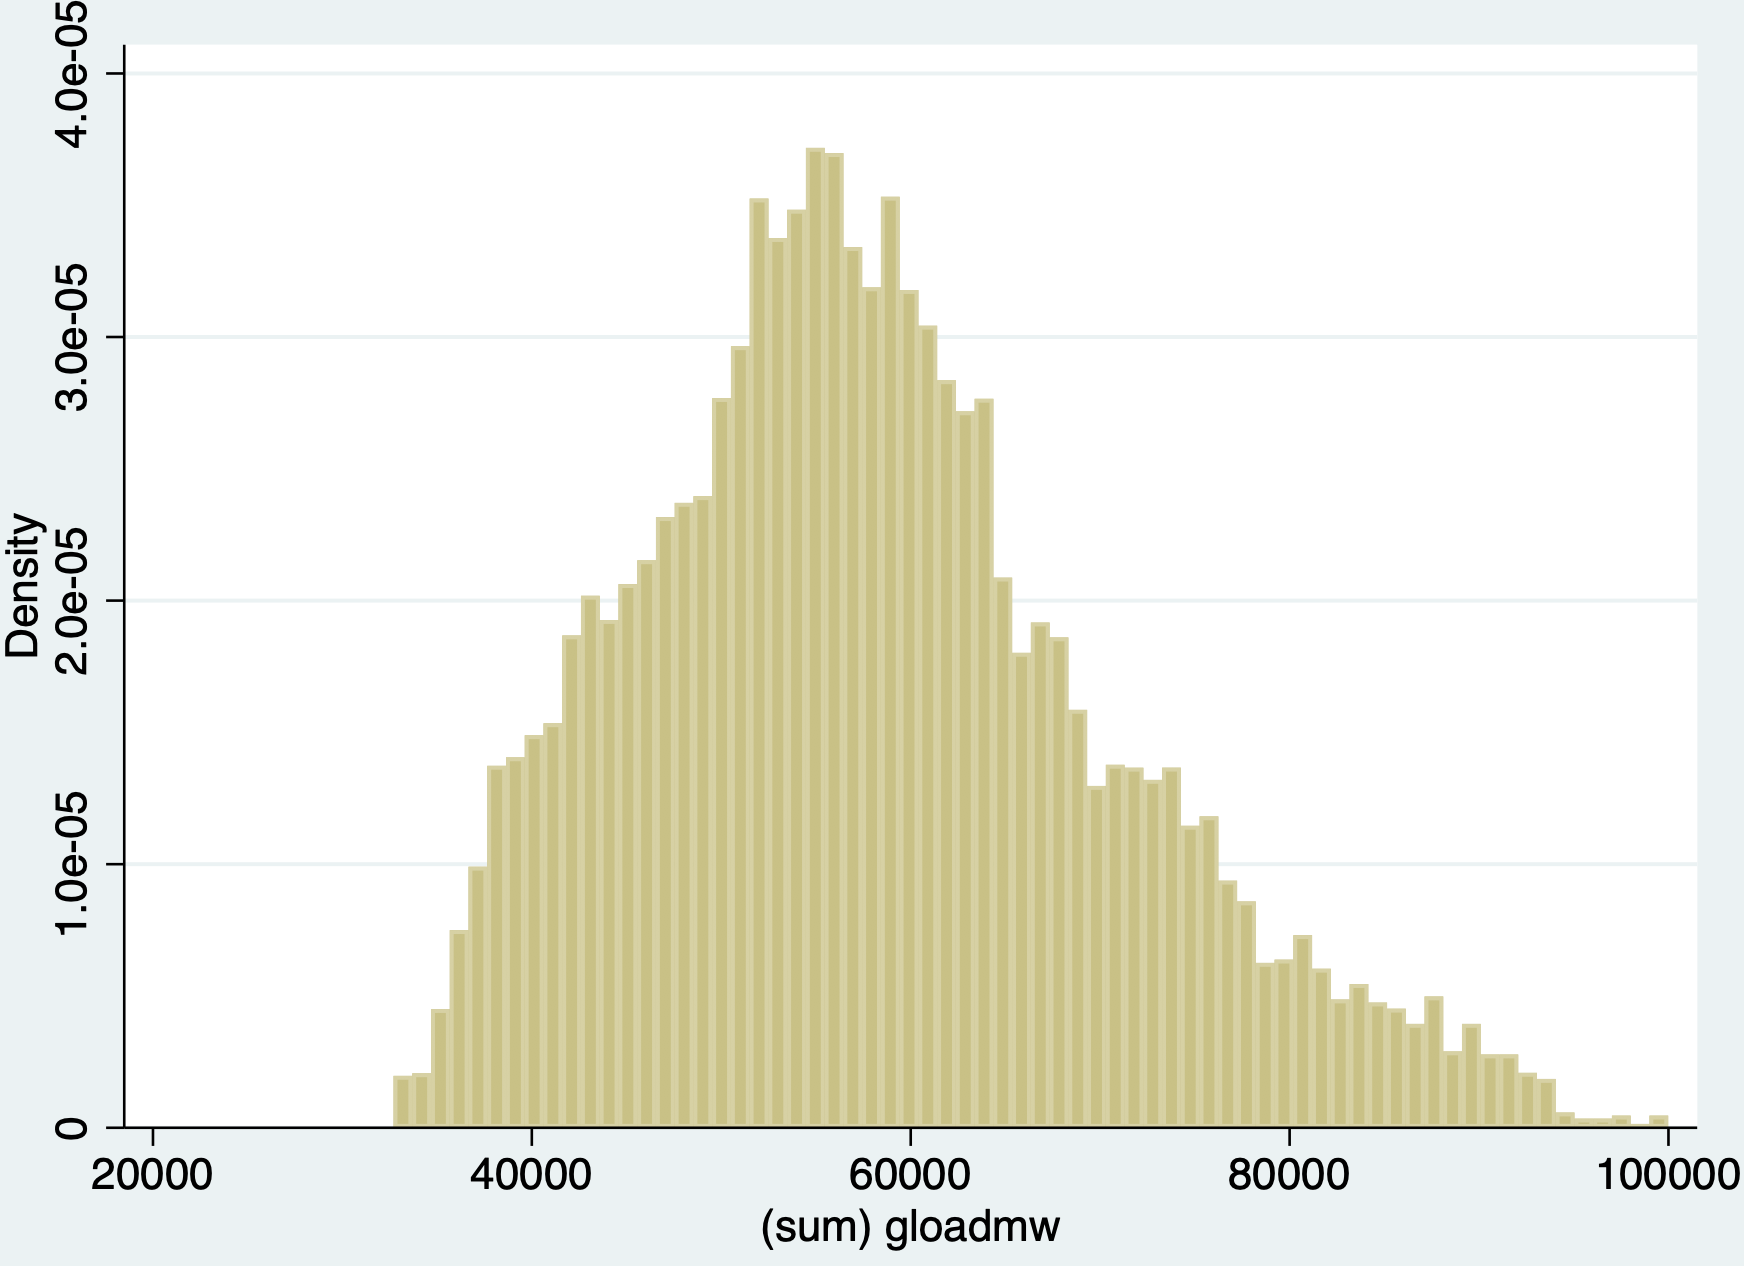
\includegraphics[width=\textwidth]{research_histogram}
%\end{columns}
%5 number summary is 
%$$32698 \hspace{10mm} 49398 \hspace{10mm} 56887 \hspace{10mm} 65381 \hspace{10mm} 99985$$
%Mean is 58135 which is greater than median, see histogram is skewed right. Big difference between third quartile and largest observation. Also a sign of some outliers to the right.
%\end{frame}


\end{document}
